%test
\section{System test}

\subsection{Force resistor test}
Vi skal have noget med en test af systemet. Jeg tænker måske noget med at teste tryk sensorere med at sætte en håndvægt på hver enkel af dem g se at det forhåbentligt giver nogenlunde det samme output. håndvægten skal også være inden for deres måleområde (range 20g to 2kg.) og så skal vi retfærdigøre at vi brugere sensore der "kun" kan måle så lidt tryk til at måle under folk som vejer +50 kg. Sikkert noget med at simon har sat modstande i systemet som øger sensorernes måling af tryk påvirkning. 


%sensor bait text fra DataAcquisition.tex
During the test of the FSR sensors, a problem occured with the FSR 406 placed under the heel of the subject. When weight were applied to the sensor it would measure the highest possible force the sensor can measure, and no useful data could be collected from the sensor. It were evaluated why this happened and discovered that because the FSR 406 covers a larger area and were placed at the heel it would be affected by more force. As the distribution of pressure is higher at the heel compared to anywhere else under the foot, it makes sense that the FSR 406 would be overloaded \cite{Hessert2005}. To account for this, the FSR 402 placed at the medial side of the feet where switched with the FSR 406 at the heel. As the FSR 402 covers a smaller area they would not be overloaded as easily as the FSR 406. As a result the FSR 406 is now placed at the medial side of the anterior eminence of the sole, and one FSR 402 is placed at the heel. The new placement of FSR sensors can be seen in \figref{fig:soleSensorPlacement}.

%THIS SHOULD BE CHANGED SO THAT THE FSR406 SENSOR IS AT THE LATERAL EMINECNE AND NOT THE MEDIAL EMINENCE OF THE SOLE!!!!!
%ALSO THE PICTURES SHOULD BE CHANGED
\begin{figure}[H]
	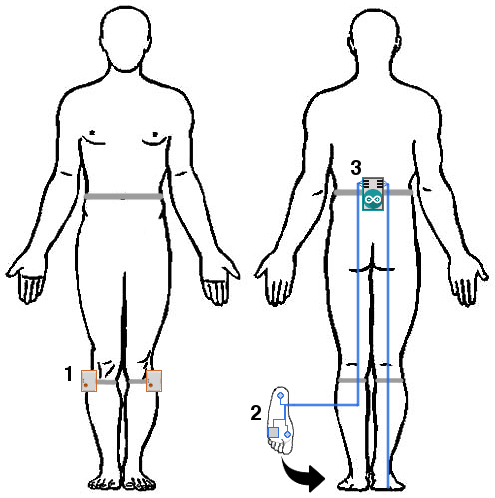
\includegraphics[width=.6\textwidth]{figures/bodySysSetup}
	\caption{The new placement of the FSR 402s and 406 under the foot of subjects.}
	\label{fig:soleSensorPlacement}  %<--remember LABEL!
\end{figure}



\subsection{Gyroscope and/or Accelerometer test}
til test af gyro/accel kan vi gøre som paul foreslog og filme personen imens de drejer rundt eller noget, hvor vi kan synkronisere film med gyro/accel målinger og se at der sker udsving på samme tidspunkt som personen drejer/bevæger sig. Det kan self ikke være med i rapporten men vi kan vise det til eksamen. 


Check that the feet are more visible than the head. 
Test walk sequence: Wait 3 sec. light jump. wait 1 sec. walk 5 steps. 180 turn. walk 5 steps. 90 turn right. wait. 90 turn right. wait. quick 180. wait quick 180. wait 1. light jump. wait 3 sec. 